%\documentclass[<options>]{elsarticle}
\documentclass [sort&compress] {elsarticle}
\usepackage{graphicx}% Include figure files

\bibliographystyle{elsarticle-num}
\begin{document}
\begin{frontmatter}

\title{Acoustically driven degradation in single crystalline silicon solar cell}

\author{O.Ya.~Olikh}
\ead{olikh@univ.kiev.ua}

\address{Faculty of Physics, Taras Shevchenko National University of Kyiv, Kyiv 01601, Ukraine}


\begin{abstract}

In this work numerical simulator SCAPS (Solar Cell Capacitance Simulator) is used to elucidate this phenomenon.

The influence of ultrasound on current--voltage characteristics of crystalline silicon solar sell was investigated experimentally.
The transverse and longitudinal acoustic waves were used over a temperature range of 290--340~K.
It was found that the ultrasound loading leads to the reversible decrease in the photogenerated current, open--circuit voltage, fill factor, carrier lifetime, and shunt resistance as well as the increase in the ideality factor.
The experimental results were described by using the models of coupled defect level recombination, Shockley--Read--Hall recombination, and dislocation--induced impedance.
The contribution of the boron-�oxygen related defects, iron-�boron pairs, and oxide precipitates to both the carrier recombination and acousto--defect interaction was discussed.
The experimentally observed phenomena are associated with the increase in the distance between coupled defects as well as the extension of the carrier capture coefficient of complex point defects and dislocations.
\end{abstract}

%\pacs{73.30.+y, 43.35.Ty, 43.35.+d, 72.20.-i, 73.40.-c}

\begin{keyword}
silicon solar cell\sep simulation\sep ideality factor\sep iron concentration
\end{keyword}

\end{frontmatter}


\section{Introduction}

It is well known that impurities are crucial for the semiconductor devices performance.
It is completely relevant to solar cell (SC) as well.
Dopants determinate an internal electric field, which leads to a separation of light-generated carriers and a photovoltage generation.
Contaminants act often as a highly effective recombination centre, reducing the carrier lifetime and SC efficiency.
Therefore the impurity concentration determination is a very important problem.
There are many experimental methods for solving this problem, such as the infrared spectroscopy, deep level transient spectroscopy, photoluminescence,
thermally stimulated capacitance and current, secondary ion mass spectrometry etc \cite{Schroder2006}.
These methods are complicated  enough and demand a special setup.

At the same time, the analysis of  the current--voltage ($I-V$)  characteristic is commonly used  to characterize the solar cell.
Thus, the dark $I-V$ curve normally serves as a first diagnosis of SC recombination \cite{Grover}.
The $I-V$  equation that models the SC by an equivalent electrical circuit contains several parameters related to physical phenomena occurring in the device.
It is obviously that these parameters depend on impurities, but the interrelations are intricate sufficiently.
As a result, $I-V$ curves are not used practically for a contaminant diagnosis, although the possibility of simultaneous calibrate both SC performance and impurity looks quite attractive.

One of a number of parameters of SC model is ideality factor $n$.
If the defect related recombination  is a prevailing process within  a  space charge region than the value $n=2$ is often stated in a literature.
But it  is  only  the  very specific  assumptions about  the  energy levels  (middle  of  the  bandgap) and  capture  cross sections  (equal for electrons and  holes)  of  the
recombination centres in a symmetrically  doped diode which lead to $n=2$ \cite{n2Kuhn,n2_Beier}.
A discrepancy between this $n=2$--theory and experiment is observed and a $n$ value depends on SC ambient conditions and the parameters of the recombination centers, particularly  their concentration \cite{n2_Beier,n2McIntosh,n2Kaminski,HAMEIRI2013251,Heide}.

The aim of our work is to investigate a possibility of  a contaminant concentration evaluation by using an ideality factor value.
The heuristic approach is used and its milestones can be expressed as following:
i)~the dark $I-V$ characteristic of the SCs with known contaminant composition is simulated;
ii)~the obtained characteristic is fitted according to the double--diode model and the ideality factor is determined;
iii)~the initial impurity concentration and the calculated ideality factor value are used for acquisition of analytic or grading dependencies.

As a first step, the paper considers a fairly simple but practically important system.
Namely, the crystalline silicon SC and iron impurity were under consideration.
Si photovoltaic device cover almost 90\% of global SC market.
Iron is a major contaminant due to the wide use of stainless steel equipment in the fabrication line and one of the most detrimental metal impurities in solar--grade crystalline silicon materials \cite{Istratov1999,FeB:Schmidt,ZHU2016192}.

Numerical simulation is carried out using the one--dimensional code SCAPS \cite{SCAPS1,SCAPS2}.
This software is widely used to modeling of various solar cells \cite{SCAPSuse1,SCAPSuse2,SCAPSuse3,SCAPSuse4,SCAPSuseSi1,SCAPSuseSi2,SCAPSuseSi3},
including silicon based devices \cite{SCAPSuseSi1,SCAPSuseSi2,SCAPSuseSi3}.

\section{Simulation details}
\subsection{Solar cell structure and material parameters}
The simple structure, which is used in the SC simulations, is  shown on inset in Fig.~\ref{figIV}.
The main used parameters are listed in Table~\ref{tabSC}.


\begin{table}
\caption{\label{tabSC}Parameters of the simulated solar cell.
}
\begin{tabular}{lcl}
\hline
\hline
Parameter&Symbol&Value\\
\hline
Emitter thickness & $d_n$ &0.5~$~\mu$m\\
Base thickness & $d_p$ &300~$~\mu$m\\
Emitter Doping (n--type, uniform)& $N_\mathrm{D}$ &$10^{19}$~cm$^{-3}$\\
Base Doping (p-type, uniform)& $N_\mathrm{A}$ &$10^{15}\div 10^{17}$~cm$^{-3}$\\
Iron content (base, uniform) & $N_{\mathrm{Fe}}$ &$10^{10}\div 10^{13}$~cm$^{-3}$\\
Temperature & $T$ &$290\div330$~K\\
%8.0&longitudinal&0.18&1.3&0.3&lUL&SC4, SC15\\
%4.2&transverse&0.19&2.8&0.6&tULa&SC15\\
%4.2&transverse&0.22&3.1&0.7&tULb&SC4\\
%4.2&transverse&0.40&4.2&0.9&tULc&SC4, SC15\\
\hline
\hline
\end{tabular}
\end{table}

In our simulation, the temperature dependencies of bandgap and carrier mobility are calculated, respectively,  according to Varshni and Caughey--Thomas equations \cite{Schroder2006}.
Bandgap narrowing is considered as described by the Slotboom equation \cite{Markvart,ZHOU20188}.
The density of states in the conduction/valence band and thermal carrier velocities are from Green \cite{Nc:Green}.

%It should be noted that the SCAPS takes into account the simplified temperature dependencies of density of states in the conduction/valence band
%($N_C$/$N_V$) and  thermal electron/hole velocity ($\upsilon_{\mathrm{th},n}$/$\upsilon_{\mathrm{th},p}$) only.

The iron atoms are known to be located in interstitial lattice position in silicon, predominantly.
The donor level $E_{\mathrm{Fe}_i} = E_V+0.394$~eV is associated with $\mathrm{Fe}_i$ \cite{Rein2,MurphyJAP2011}.
Therefore neutral  interstitial  iron  $\mathrm{Fe}_i^0$ and interstitial ionized iron $\mathrm{Fe}_i^+$   are observed in  Si.
In $p$--type material, $\mathrm{Fe}_i^+$ readily interacts with ionized shallow acceptors.
In our simulation, the boron is a dopant impurity and the pair $\mathrm{Fe}_i\mathrm{B}_s$ must be under consideration.
On the one hand, this pair is bistable defect and the trigonal and the orthorhombic configuration are feasible.
On the other hand, the orthorhombic pair is only observable at low temperature ($<150$~K) under an illumination or carrier injection condition \cite{Narland,Sakauchi}.
Besides  the $\mathrm{Fe}_i\mathrm{B}_s$ pairs can be readily dissociated by 15 to 90~s illumination with a halogen lamp \cite{FeB:Schmidt}.
The association reaction is diffusion limited and can take place under dark condition during tens minute \cite{FeB:kinetic}.
Two following cases are under simulation.


\noindent
i)~All iron atoms are isolated interstitial:
\begin{equation}
\label{eqN1}
    N_{\mathrm{Fe}}=N_{\mathrm{Fe}_i^0}+N_{\mathrm{Fe}_i^+} \,,
\end{equation}
where
$N_{\mathrm{Fe}_i^0}$ and $N_{\mathrm{Fe}_i^+}$ are the concentrations of  neutral and ionized iron respectively.
Such condition is realisable  after illumination immediately.
The interstitial iron is considered as uniform in the SC base,
the hole and electron capture cross--sections of defect are calculated according to
$\sigma_{p,\mathrm{Fe}_i}=3.85\times10^{-16}\exp(-0.045/kT)$~cm$^2$ and
$\sigma_{n,\mathrm{Fe}_i}=9.1\times10^{-15}\exp(-0.024/kT)$~cm$^2$ \cite{Istratov1999,Rein2,MurphyJAP2011}.
$E_{\mathrm{Fe}_i}$ is taken as the temperature independent value \cite{Kohno}.
This case is labeled ``FI'' from now on.

\noindent
ii)~The total dissolved iron concentration is given by a sum of concentrations of three separate species, $\mathrm{Fe}_i^0$, $\mathrm{Fe}_i^+$,
and iron paired with an boron:
\begin{equation}
\label{eqN2}
    N_{\mathrm{Fe}}=N_{\mathrm{Fe}_i^0}+N_{\mathrm{Fe}_i^+}+N_{\mathrm{FeB}}=N_{\mathrm{Fe}_i}+N_\mathrm{FeB} \,,
\end{equation}
where
$N_\mathrm{FeB}$ is the pair concentration,
$N_{\mathrm{Fe}_i}$ is the concentration of unpaired interstitial iron.
This case corresponds to an equilibrium condition.
The equilibrium concentration of $\mathrm{Fe}_i^+$  is given by \cite{MurphyJAP2011,FeB:kinetic}
\begin{equation}
\label{eqNFe+}
    N_{\mathrm{Fe}_i^+}=\frac{N_{\mathrm{Fe}}}{\left[1+N_\mathrm{A}10^{-23}\exp\left(-\frac{E_b}{kT}\right)\right]\left[1+\exp\left(-\frac{F-E_{\mathrm{Fe}_i}}{kT}\right)\right]}\,,
\end{equation}
where
$F$ is the Fermi level,
$E_b$ is the binding energy of the FeB pairs (taken as 0.582 eV).
Since the $\mathrm{Fe}_i^0$  species are  in local  equilibrium with both  isolated $\mathrm{Fe}_i^+$  atoms  and
$\mathrm{Fe}_i^+$ atoms which  are  associated in the FeB--pairs, the following expression silicon may be written as \cite{FeB:kinetic}
\begin{equation}
\label{eqNrel}
    \frac{N_{\mathrm{FeB}}+N_{\mathrm{Fe}_i^+}}{N_{\mathrm{Fe}_i^0}}=\exp\left(-\frac{F-E_{\mathrm{Fe}_i}}{kT}\right) \,.
\end{equation}
A simple transformation of Eqs.~(\ref{eqN2})--(\ref{eqNrel}) enables one to obtain the following expression for relationship between total iron concentration and pair concentration
\begin{equation}
\label{eqNFeB}
    N_{\mathrm{FeB}}=N_{\mathrm{Fe}}\frac{N_\mathrm{A}10^{-23}\exp\left(-\frac{E_b}{kT}\right)}
     {\left[1+N_\mathrm{A}10^{-23}\exp\left(-\frac{E_b}{kT}\right)\right]\left[1+\exp\left(-\frac{F-E_{\mathrm{Fe}_i}}{kT}\right)\right]}\,.
\end{equation}
The Fermi level position is not uniform in the SC base.
Hence FeB pair concentration is not uniform as well even if iron content is uniform.

In our simulation, the Fermi level position in the SC base Has been calculated for each doping and temperature values.
Then Eq.~\ref{eqNFeB} was used to calculate the FeB pair distribution.
The representative example of calculation is shown in Fig.~\ref{figDist}.

\begin{figure}
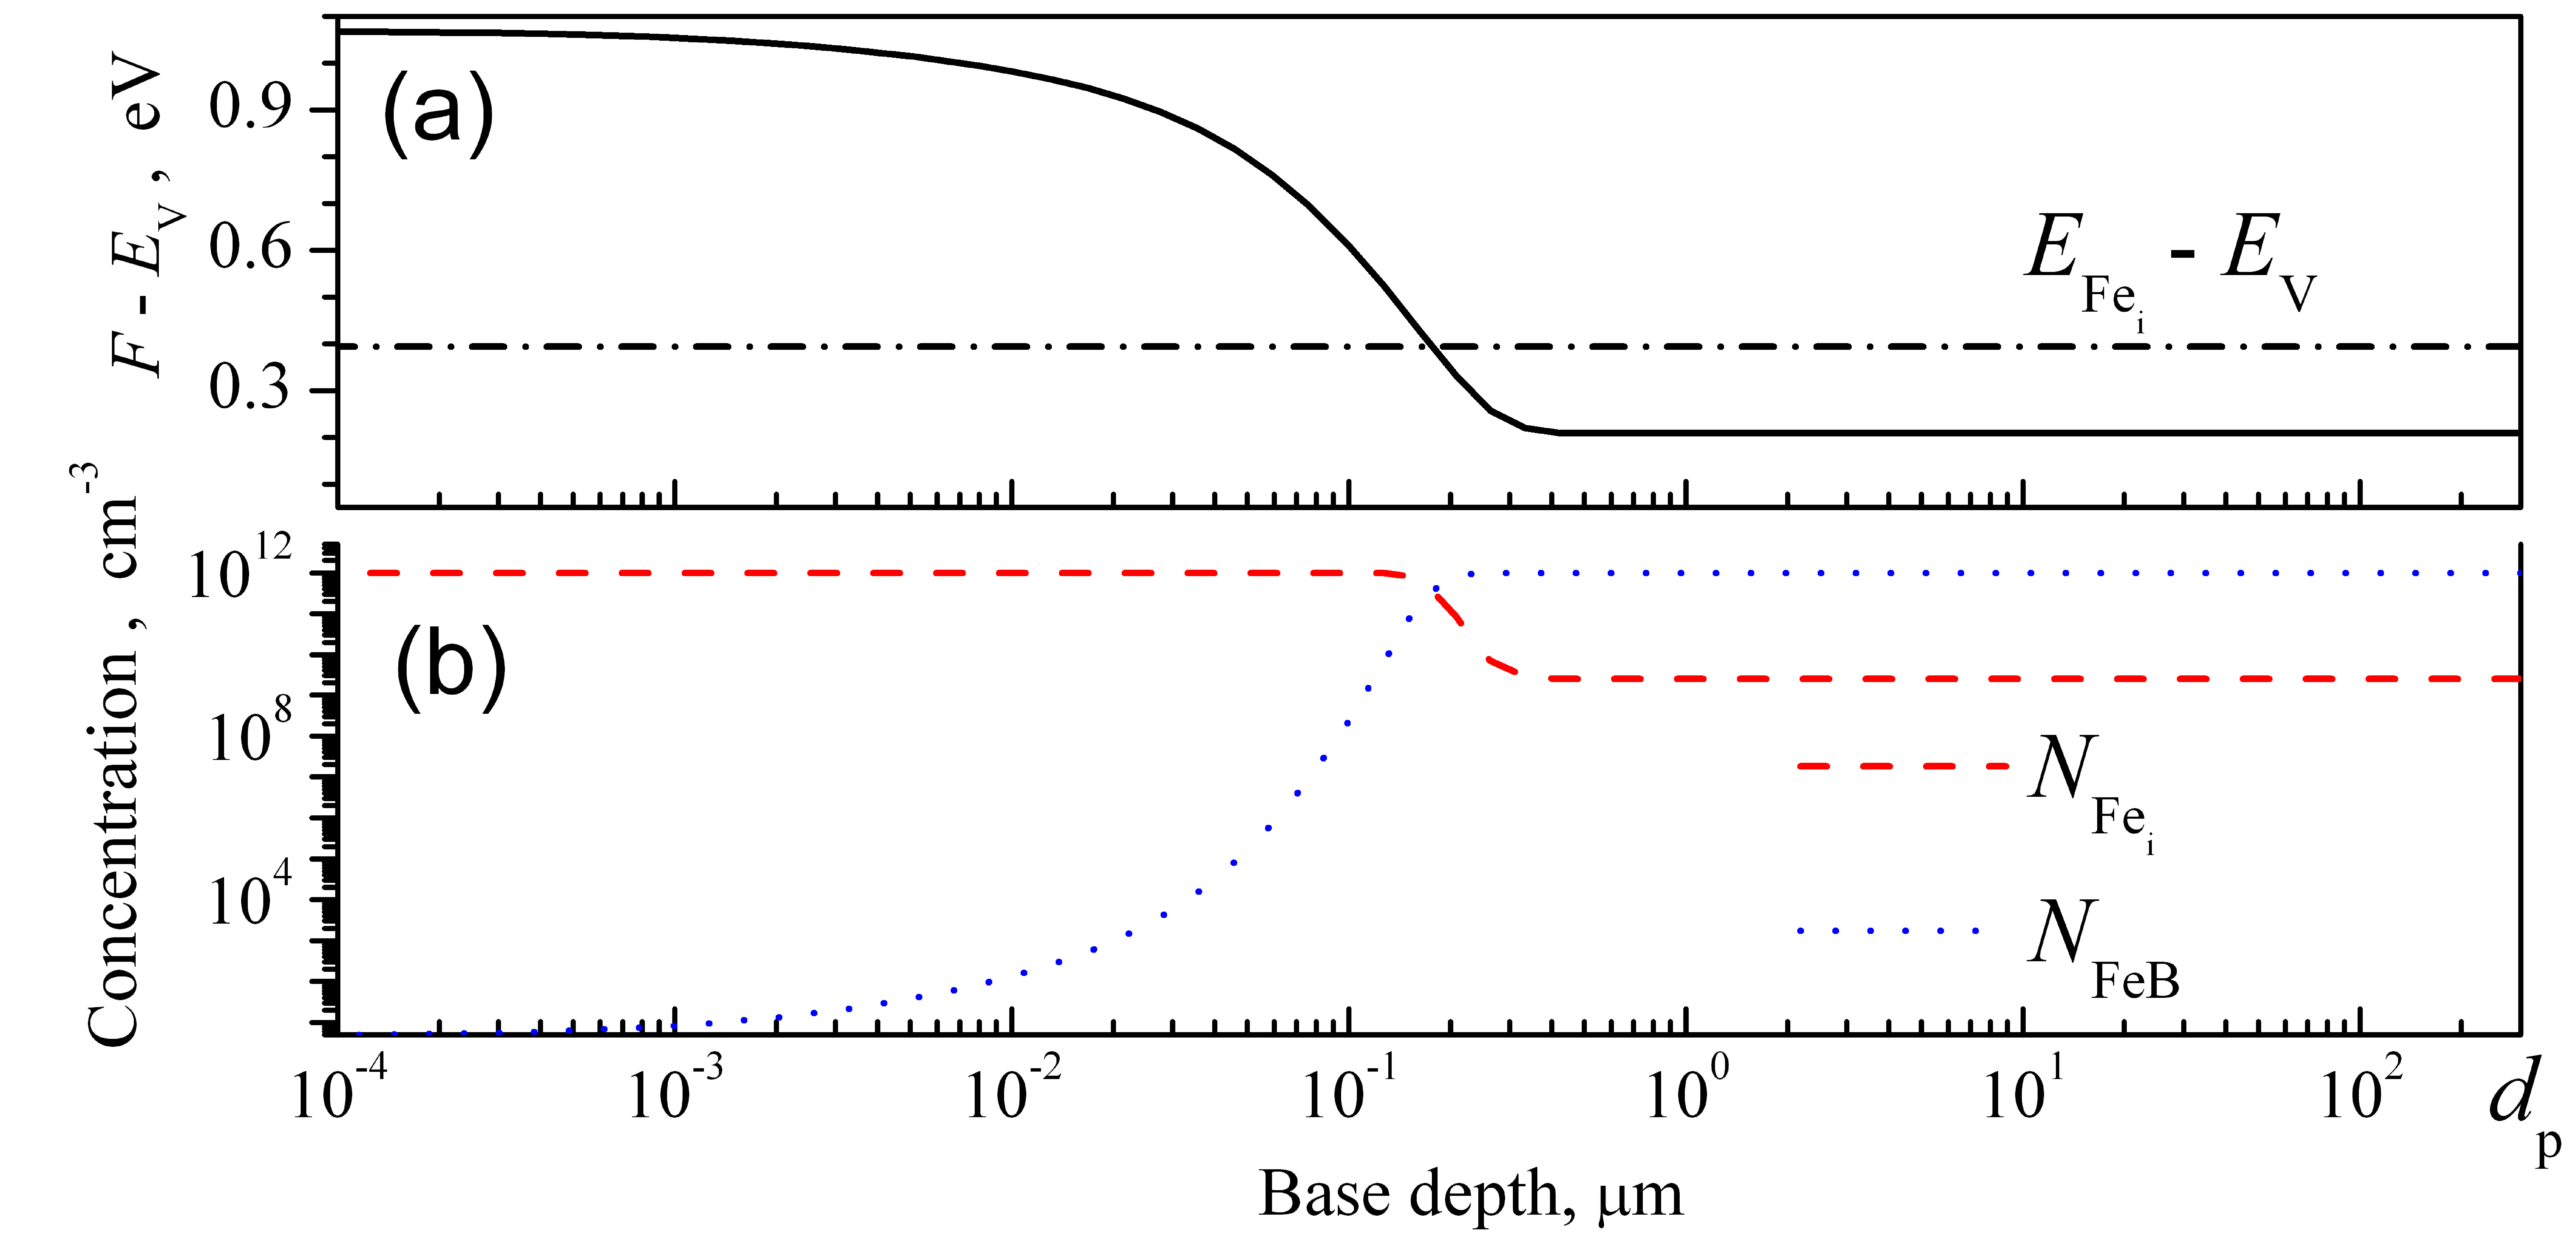
\includegraphics[width=12cm]{Fig2}%
\caption{\label{figDist}
The calculated SC base distribution of Fermi level position (a, solid line), unpaired interstitial iron concentration (b, dashed line),
and FeB pair concentration (b, dotted--dashed line).
$N_\mathrm{A}=10^{16}$~cm$^{-3}$, $T=300$~K.
The position of $\mathrm{Fe}_i$ donor level (dotted line) is shown in the panel (a) as well.
}%
\end{figure}

The trigonal configuration of the FeB pair is considered.
This pair is amphoteric defect.
In our simulation, the parameters of donor ($E_{\mathrm{FeB}}^{d} = E_V+0.10$~eV,
$\sigma_{p,\mathrm{FeB}}^d=2\times10^{-14}$~cm$^2$,
$\sigma_{n,\mathrm{FeB}}^d=4\times10^{-13}$~cm$^2$)
and  acceptor ($E_{\mathrm{FeB}}^{a} = E_C-0.26$~eV,
$\sigma_{p,\mathrm{FeB}}^a=5.5\times10^{-15}$~cm$^2$,
$\sigma_{n,\mathrm{FeB}}^a=2.5\times10^{-15}$~cm$^2$)
levels are used from \cite{Istratov1999,Rein2,MurphyJAP2011,FeB:kinetic}.
This case is labeled ``FIFB'' from now on.

Only a bulk recombination is under consideration in the paper.
Once again two cases are simulated.
In the first one, labeled ``SRH'', the Shockley--Read--Hall recombination is taken into account only.
In the second one, denoted ``SRHBBA'', the both Shockley--Read--Hall recombination and intrinsic recombination are allowed for.
The electron and hole Auger recombination factors and radiative band--to--band recombination coefficient are taken from \cite{Markvart}.

So, four different data sets (FI--SRH, FI--SRHBBA, FIFB--SRH, and FIFB--SRHBBA) 
have been simulated for solar cell.


\begin{figure}
%\begin{center}
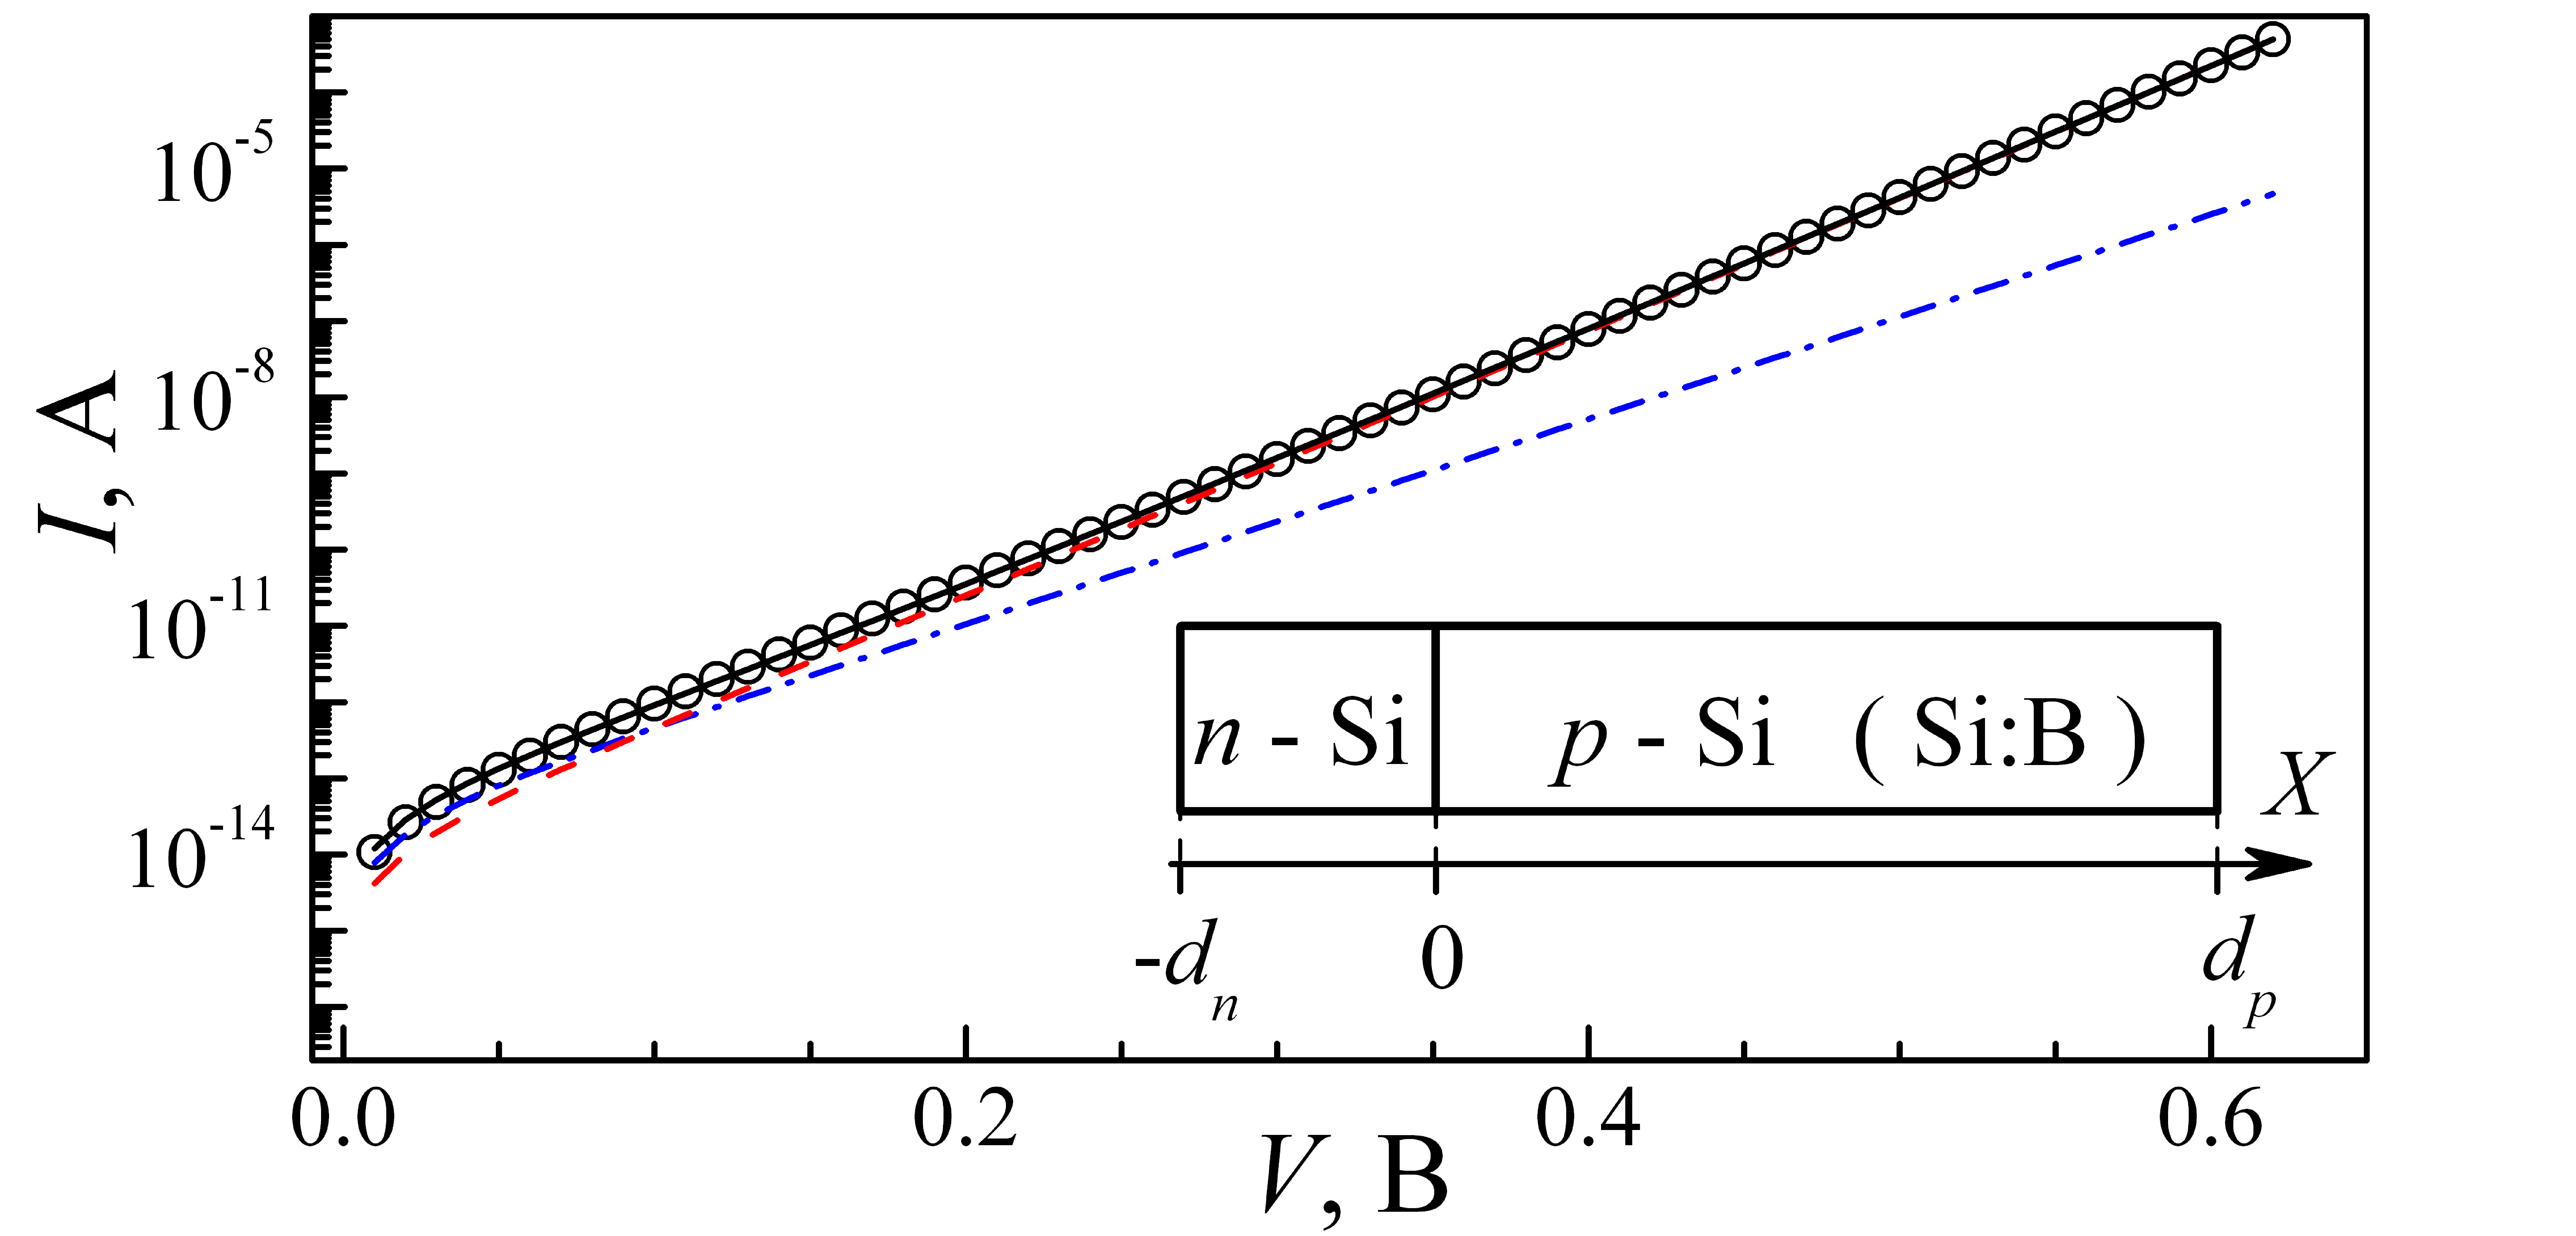
\includegraphics[width=12cm]{Fig1}%
%\end{center}
\caption{\label{figIV}
$I-V$ characteristic simulated in FI--SRH--case, $N_\mathrm{A}=10^{17}$~cm$^{-3}$,  $N_{\mathrm{Fe}}=10^{13}$~cm$^{-3}$, $T=290$~K (marks)
and its fitting by Eq.~(\ref{eqIV}) (solid line).
The dashed and dotted--dashed lines represent the diffusion and recombination currents.
Inset: Solar cell structure, which are used in simulation.
}%
\end{figure}

The dark forward $I-V$ characteristic were generated by SCAPS over a voltage range up to $0.62$~V.
The $I-V$ curve example is shown in Fig.~\ref{figIV}.

The real silicon SCs are described by so--called two--diode model.
The first diode represents the ``ideal'' diode, describing the so--called diffusion current, characterized by a saturation current $I_{01}$, 
and the second diode is the so--called recombination current, characterized by a saturation current $I_{02}$ and an ideality factor $n$ \cite{Breitenstein2013}. 
According to the two--diode model, the dark SC current is given by
\begin{equation}
\label{eqIV}
    I=I_{01}\left[\exp\left(-\frac{qV}{kT}\right)-1\right]+ I_{02}\left[\exp\left(-\frac{qV}{nkT}\right)-1\right]\,.
\end{equation}
It should be noted that the influence of series resistance as well as shunt resistance is neglected in Eq.~\ref{eqIV}.
We used Eq.~\ref{eqIV} to fit the simulated data taking $n$, $I_{01}$, and $I_{02}$ as the fitting parameters.
The fitting result is shown in Fig.~\ref{figIV}.

All non-linear fittings in the paper were done by using the differential evolution method \cite{DE:Sun,DEWang}.
The least--squares method was used to linear fitting.



%We have used two approaches to calculate the depletion region. The first approach is based
%
%In the following analysis, Teff is considered approximately equal to 1, a true condition for quasi-ballistic devices.
%
%Fig. 5 displays themeasured TCs of the FF of the studied cells and that of record silicon cells together with a generic theoretical calculation (green line) and speci?c theoretical predictions based on experimental values for each cell (triangles).
%
%In our simulation, themodel for dopant ionization is from Altermatt et al. [18]. The intrinsic carrier concentration is calculated according to models from Couderc et al. [19]. The bandgap and bandgap narrowing models are, respectively, from Passler [20] and Yan and Cuevas [21]. The thermal velocity is calculated from models by Green [22]. (IEEEJPhotovol_7_p1092-1097.pdf)
%
%we also assume a negligible proportion of Fe present in the form of FeB pairs (a safe assumption for cells operating under constant illumination)
%ProgPVResAppl_8_p363.pdf
%
%FeB pairs can be reversibly dissociated either by a thermal anneal of the samples at 200 C for 10min followed by a quench, or by 15 to 90 s illumination with a halogen lamp.
%PR_Istratov_obzor2_ApplPhysA_70_p489_534.pdf
%
%In this work, the electrical parameters of a silicon solar cell are investigated theoretically using a one dimensional model
%
%The intrinsic recombination can be subdivided into radiative and Auger recombination
%
%20. Bandgap narrowing is considered as described by the Slotboom equation [24]:
%(MatSciSemProc_86_p8.pdf,  D:\Literat\Stat\IVchar\PN\Manufacturing\)

%Applying this model, a virtual population of 500 I�V
%curves whose two-diode parameters (JL, J01, J02, Rs, Rp)
%are randomly chosen into representative ranges for crystal-
%line silicon-based solar cells is generated (see [15] and the
%references therein).




\section{Results and Discussion}
\subsection{Interstitial iron, SRH recombination}








\section{Conclusion}
The influence of ultrasound on the silicon solar cell  has been investigated experimentally over a temperature range of 290--340~K.
The investigation has revealed an acoustically driven reversible degradation in SSC parameters.
The effect is intensified in the case of the transverse acoustic waves using.
The analysis has shown that degradation is caused by the acoustically induced increase in the carrier capture coefficient for point or extended defects.
The qualitative model of the observed phenomenon, which is based on the increase in the distance between coupled defects or between complex defect components due to ultrasound action, has been considered.
It has been shown that the oxide precipitates are most likely defects, which take part in the acousto--defect interaction.
Thus, ultrasound can be an effective tool for controlling silicon structure characteristics.



\section*{References}

\bibliography{olikh}

\end{document}

